\section{The Optimization Problem}

In much of mathematics, our goal is to seek some sort of solution. In cases where there are multiple solutions, it is desirable to determine the ``best'' solution judged against some set of criteria. Mathematical optimization is the study of solving such problems. In its simplest case, mathematical optimization is the practice of minimizing or maximizing a given function over a certain set and possibly subject to some constraints.

\begin{defn}
	An optimization problem (in standard form) has the form
	\begin{equation}
		\begin{tabular}{lll}
			\text{minimize }   & $f_0(x)$        &                 \\
			\text{subject to } & $f_i(x)\leq 0$, & $i=1,\ldots, m$ \\
			& $h_i(x) = 0$,   & $i=1,\ldots, p$ 
		\end{tabular}\label{Optimization}
	\end{equation}
	where
	\begin{itemize}
		\item $x=\left(x_1,\ldots,x_n\right)$ are the optimization variables,
		\item $f_0 : \mathbb{R}^n\rightarrow\mathbb{R}$ is the objective function,
		\item $f_i : \mathbb{R}^n\rightarrow\mathbb{R}$ are the inequality constraint functions, and
		\item $h_i : \mathbb{R}^n\rightarrow\mathbb{R}$ are the equality constraint functions.
	\end{itemize}
\end{defn}
If there are no constraints ($m=p=0$), then the problem is called \textit{unconstrained}. \cite[p. 127]{Boyd2004}

We call a vector $x^\star$ \textit{globally optimal} if it has the smallest objective value among all vectors that satisfy the constraints. That is, for any $z$ with $f_1(z)\leq 0,\ldots, f_m(z)\leq 0$, then $f_0(z)\geq f_0(x^\star)$. A point $x$ that is in the domains of each function $f_i$ and $h_i$ is called \textit{feasible} if it satisfies all the constraints. Finally, the \textit{optimal value} $p^\star$ of the problem is defined as $$p^\star=\left\lbrace f_0(x) \mid f_i(x)\leq 0, i=1,\ldots,m, h_i(x)=0, i=1,\ldots,p\right\rbrace.$$ Therefore, $p^{\star}=f_0(x^\star)$, the objective function value at a feasible and globally optimal vector $x^{\star}$.

Notice that the optimization problem in standard form is a minimization problem.  We can easily change it into a maximization problem by minimizing the objective function $-f_0$ subject to the same constraints.

The optimization problem is \textit{linear} or called a \textit{linear program} if the objective and constraint functions are all linear. An optimization problem involving a quadratic objective function and linear constraints is \textit{quadratic} or a \textit{quadratic program}. If the optimization problem is not linear or quadratic, it is referred to as a \textit{nonlinear program}.

There are exists efficient methods for solving linear programming and many quadratic programming problems.

\subsection{Convex Optimization}

A set $C$ is \textit{convex} if the line segment between any two points in $C$ lies in $C$. That is if for any $x_1,x_2\in C$ and any $\theta$ with $0\leq\theta\leq 1$, we have $\theta x_1+(1-\theta)x_2\in C$.

A function $f : \mathbb{R}^n\rightarrow\mathbb{R}$ is convex if the domain of $f$ is a convex set and if for all $x,y$ in the domain of $f$, and $\theta$ with $0\leq\theta\leq 1$, we have
\begin{equation}
	f\left(\theta x+\left(1-\theta\right)y\right)\leq\theta f(x)+(1-\theta)f(y).
	\label{eqn:Convexity}
\end{equation}
A \textit{convex optimization problem}, therefore, is an optimization problem of the form
\begin{equation}
	\begin{tabular}{lll}
		\text{minimize }   & $f_0(x)$        &                 \\
		\text{subject to } & $f_i(x)\leq 0$, & $i=1,\ldots, m$ \\
		& $a_i^T = b_i$,  & $i=1,\ldots, p$ 
	\end{tabular}\label{ConvexOptimization}
\end{equation}
where $f_0,\ldots,f_m$ are convex functions.

Notice that there are three requirements that differentiate a convex optimization problem from a general optimization problem:
\begin{itemize}
	\item the objective function must be convex
	\item the inequality constraint functions must be convex
	\item the equality constraint functions must be affine
\end{itemize}

In a convex optimization problem we minimize a convex objective function over a convex set and any locally optimal point is also globally optimal. This is a \textit{very} useful fact!

Why might local optimality implying global optimality be useful? Consider a situation where we have a convex objective function. If we are able to find any minimum value for the objective function, then we know this value is not just a local minimum, but indeed a global minimum. If we do not have a convex function, we cannot be as assured that we have found the global optimal value. For example, consider a function such as the one shown in \figref{fig:non-convex-function-example}. An optimization strategy may find the local minimum near $x=1$, but since the function is not convex everywhere on its domain, we cannot conclude that this value is the truly optimal value. In fact, we see that the global minimum, and hence the actual optimal value, is between $x=-1$ and $x=-0.5$. On the other hand, if we have a function that is everywhere convex, as soon as we find a local minima, we can be assured that it is also the global minima!

\begin{figure}
	\centering
	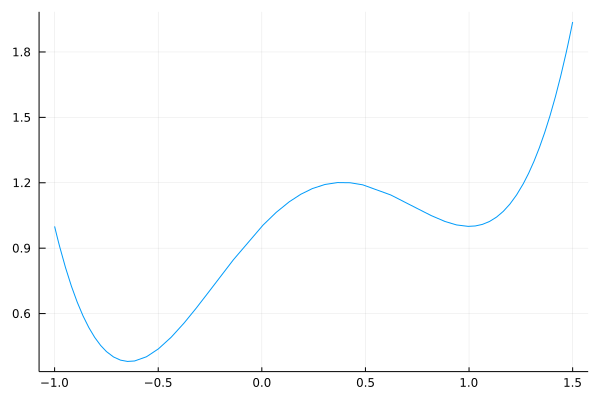
\includegraphics[width=0.8\textwidth]{Chapter_I_Background/Images/Non-Convex-Example.png}
	\caption[A Non-Convex Function]{A graph of the non-convex function $f(x)=x^4-x^3-x^2+x+1$. Notice it has two local minima and that the right local minima is not equal to the global minimum.}
	\label{fig:non-convex-function-example}
\end{figure}

So we can see that convexity is a very powerful and useful property in terms of optimization problems. As a result, any time we can take advantage of convexity or approximate functions using convex functions, we often do so.